%!TEX root = problems.tex

%\printanswers

\noindent
The following problem was first presented by Leonhard Euler~\cite{euleroriginal}.
The problem concerns a former city called Königsberg, which is now called Kaliningrad, in Prussia (now in Russia).
Take the time to try to solve this problem yourself.

\subsubsection*{Question}
In Königsberg, there were seven bridges linking four different parts of the city.
These are depicted in the diagram below.
The question is: is it possible to walk through the city crossing each bridge once and only once~\cite{konigsbergwikipedia}?

\begin{center}
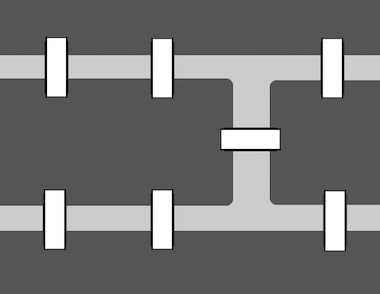
\includegraphics{diagram}
\end{center}